\section{Evaluation} \label{eval}
In this section, we evaluate the \sys prototype on the physical RDMA platform. In addition to the basic network performance, such as throughput and latency, it also includes the real-world RDMA application. We expect to answer the following questions:
(1) Can \sys's network performance in container and virtual machine be both close to native RDMA?
(2) Can \sys be adapted to the real-world RDMA application in containers or virtual machines?

\subsection{Experiment Methodology}
All experiments are carried out on two servers. The settings mainly include three parts: host server, container and virtual machine. 

The RNIC used by the server is Mellanox ConnectX-3 56 Gb/sec, which performs RDMA communication under Infiniband. For host servers, the operating system is all CentOS 7.4.1708 (Linux 3.10.0-693.el7.x86\_64). The RDMA driver installed on the host server is Mellanox OFED 4.4-2.0.7.0~\cite{mlnx-ofed}. To get consistence, virtual machines and containers are built based on the same OS images as host. All virtual machines are based on QEMU(5.1.50)~\cite{qemu} enabled with KVM~\cite{kvm} and the container engines are Docker(18.06.1-ce)~\cite{docker}. In addition, the entire \sys framework is compiled with GCC/G++ 4.8.5, and the O3 compilation optimization level is selected. 

\subsection{Basic benchmark}
Throughput and latency are the key target of network performance. RDMA supports two different data transmission modes: unilateral and bilateral. Due to the difference performance between them, we evaluate them respectively.

Based on the RDMA benchmark test tool perftest~\cite{perftest}, we evaluated the throughput and latency of \sys, native RDMA, hardware virtualization SR-IOV, and software virtualization FreeFlow in virtual machines or containers. For two-sided operations (Send and Recv), we use the ``ib\_send\_bw'' and ``ib\_send\_lat'' commands; for one-sided operations (Write and Read), with Write as the representative, we use the ``ib\_write\_bw'' and ``ib\_write\_lat'' commands. The specific process is: after the RDMA connection is established between the client and the server, the bytes of transmitted message each time will be increased from 4B to 1MB, the data will be iteratively transmitted 1000 times with each message size, and finally the average throughput and latency are calculated.

(1) Throughput: The results of bilateral operation are shown in Figure~\ref{fig:send-bw}, and the one of unilateral operation are shown in Figure~\ref{fig:write-bw}. Whether \sys is in a virtual machine or in a container scenario, the throughput of its bilateral and unilateral operations is similar as SR-IOV and close to native RDMA.

Compared with FreeFlow, when the message is small, the throughput of \sys has reached 4-6 times that of FreeFlow. Because FreeFlow forwards all data commands to the software virtualization layer for processing. Therefore, the forward latency gradually accumulates and decrease the throughput significantly. However, \sys maps all RDMA resources to execute data commands in the user space of the container or virtual machine. Therefore, there is no latency for commands forwarding in data path.

\begin{figure}[!ht]
	\centering
	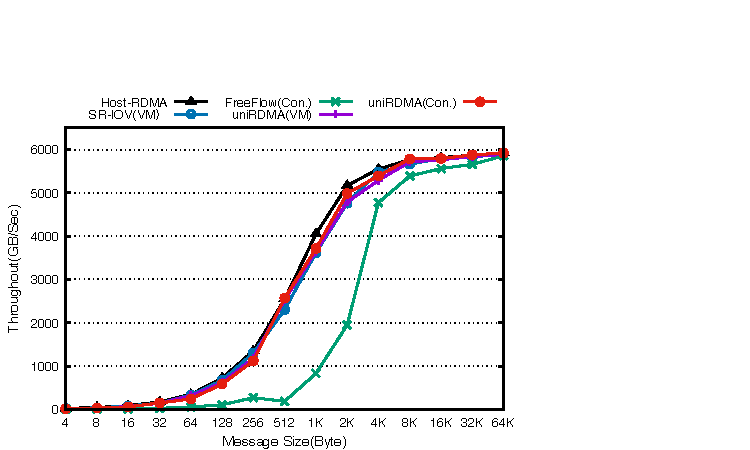
\includegraphics[width=1.0\linewidth]{images/send-bw.pdf}
	\caption{The Throughout of RDMA Send and Recv}
	\label{fig:send-bw}
\end{figure}

\begin{figure}[!ht]
	\centering
	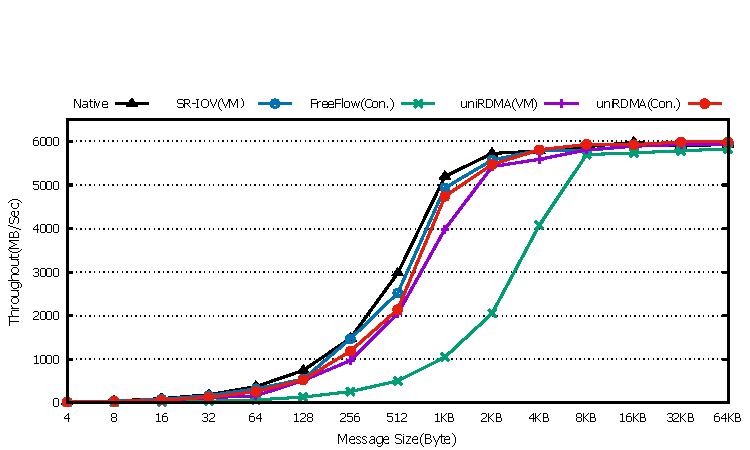
\includegraphics[width=1.0\linewidth]{images/write-bw.pdf}
	\caption{The Throughout of RDMA Write}
	\label{fig:write-bw}
\end{figure}

When the message gradually increases, such as reaching 64KB, the throughput of each framework tends to be consistent. The reason is that the bandwidth is saturated, and the delay overhead of FreeFlow has been covered by waiting delay in RNIC.

(2) Latency: The results of bilateral operation are shown in Figure~\ref{fig:send-lat}, and the one of unilateral operation are shown in Figure~\ref{fig:write-lat}. Whether \sys is in a virtual machine or in a container scenario, the latency of its bilateral and unilateral operations is similar as SR-IOV and close to native RDMA.

Compared with FreeFlow, when the message is small, the latency of \sys has reached 40\%~60\% of FreeFlow because of FreeFlow's forwarding latency. Also, when the message gradually increases, such as reaching 64KB, the latency of each framework tends to be consistent. Because the main latency has been caused by RNIC data processing.

\begin{figure}[!ht]
	\centering
	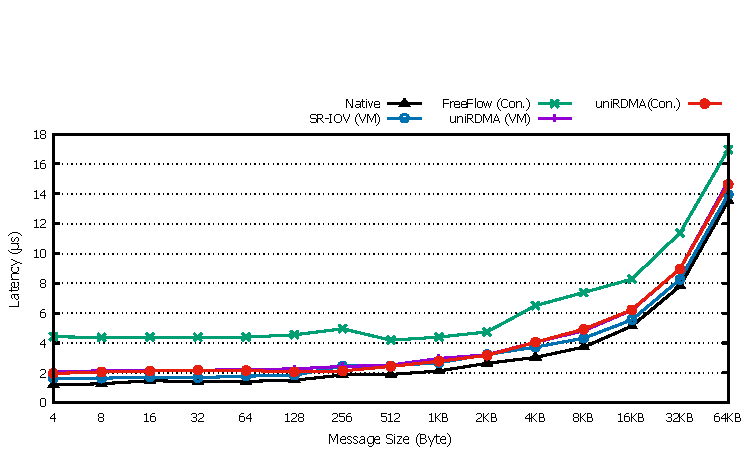
\includegraphics[width=1.0\linewidth]{images/send-lat.pdf}
	\caption{The Latency of RDMA Send and Recv}
	\label{fig:send-lat}
\end{figure}

\begin{figure}[!ht]
	\centering
	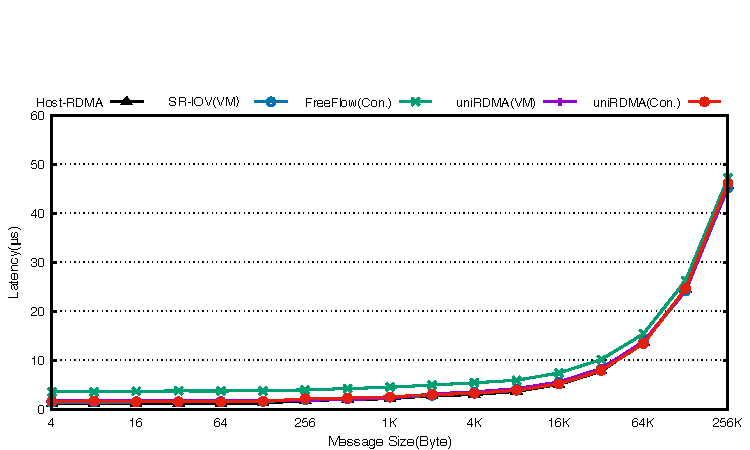
\includegraphics[width=1.0\linewidth]{images/write-lat.pdf}
	\caption{The Latencty of RDMA Write}
	\label{fig:write-lat}
\end{figure}

\subsection{Real-world Applications}

The worth of RDMA is mainly about its optimized performance in real-world applications. RDMA virtualization needs to maintain the performance close to native RDMA. Therefore, we evaluate \sys and other frameworks in high-performance computing benchmark Graph-500. Graph-500 is a benchmark framework used to test the performance of the Message Passing Interface (MPI). Based on the constructed graph structure, users test the performance of breadth-first search (BFS) and single source shortest path (SSSP). The performance index is the number of edges traversed per second (traversed edges). per second, TEPS), the larger the value, the better the performance.

In this paper, the node scale of the computational graph in Graph-500 is set to 26, and the ratio of edges to points is set to the default parameter of 16. The constructed graph has a total of 2$^{25}$ vertices, with 2$^{29}$ edges, the entire graph occupies approximately around 16GB. When testing BFS and SSP, 16 MPI processes are scattered and executed on two nodes in turn, and the average value is taken according to the results of 12 tests. The data obtained is shown in Table Figure~\ref{fig:graph-500} (because there are core dump problems when using FreeFlow for Graph-500, the corresponding data is lacking).

As shown in Figure~\ref{fig:graph-500},  the performance of \sys is close to native RDMA. Because \sys bypasses the kernel and virtualization layer in the data path, and there is no forwarding latency.

\begin{figure}[!ht]
	\centering
	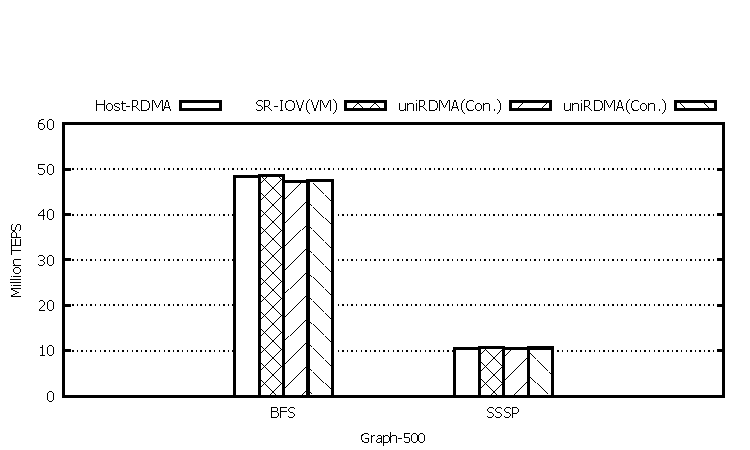
\includegraphics[width=1.0\linewidth]{images/graph-500.pdf}
	\caption{The Performance of Graph-500}
	\label{fig:graph-500}
\end{figure}